\documentclass{report}
\usepackage[margin=1in, paperwidth=8.5in, paperheight=11in]{geometry}
%Math packages%
\usepackage{amsmath}
\usepackage{amsthm}
%Spacing%
\usepackage{setspace}
%Package to adjust indentation%
\usepackage{changepage}
\onehalfspacing
%Lecture number%
\newcommand{\lectureNum}{18}
%Variables - Date and Course%
\newcommand{\curDate}{March 14, 2017}
\newcommand{\course}{CS 240}
%Defining the example tag%
%\theoremstyle{definition}%
\newtheorem{ex}{Example}[section]
%Setting counter given the lecture number%
\setcounter{chapter}{\lectureNum{}}
%Package to insert code%
\usepackage{listings}
\usepackage{courier}
\usepackage{xcolor}
\lstset { 
    tabsize=2,
    breaklines=true,
    language=C++,
    backgroundcolor=\color{blue!8}, % set backgroundcolor
    basicstyle=\footnotesize\ttfamily,% basic font setting
}
%Package to draw trees%
\usepackage{tikz}


\begin{document}
%Note title%
\begin{center}
\begin{Large}
\textsc{\course{} | Lecture \lectureNum{}}
\end{Large}
\end{center} 
\noindent \textit{Bartosz Antczak} \hfill
\textit{Instructor: Eric Schost} \hfill
\textit{\curDate{}}
\rule{\textwidth}{0.4pt}

% Actual Notes%
\section{KMP Algorithm}
Just like the brute-force method, this compares the pattern to the text from \textit{left-to-right}; however, it shifts the pattern more intelligently than the brute-force counterpart.
\subsection{Implementation}
Suppose we have a match up to position T[i-1] = P[j-1], but not at the next position. We define F[j-1] as the index we will have to check in P, after we bring the pattern to its next possible position. We shift the pattern by F[j-1] unites.
\begin{ex}
Constructing F[j] using a pattern P = abacaba
\end{ex}
\begin{center}
\begin{tabular}{ c | c | c }
\hline
j & P[0 ... j] & F[j] \\\hline
0 & a & 0 \\
1 & ab & 0 \\
2 & \underline{a}b\underline{a} & 1 \\
3 & abac & 0 \\
4 & \underline{a}bac\underline{a} & 1 \\
5 & \underline{ab}ac\underline{ab} & 2 \\
6 & \underline{aba}c\underline{aba} & 3 \\
\end{tabular}
\end{center}
\begin{figure}[ht]
\begin{center}
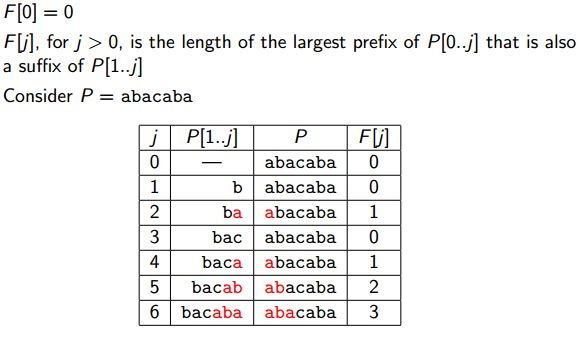
\includegraphics[scale=0.4]{kmp1.jpg}
\end{center}
\end{figure}
\subsection{KMP Analysis}
When constructing the \textbf{failure array}, there are no more than $2m$ iterations of the while loop, so it takes a time of $\Theta(m)$, where $m$ is the length of the pattern string.\\
When running the KMP algorithm, there are no more than $2n$ iterations of the while loop, so the running time is $\Theta(n)$, where $n$ is the length of the text for which we're finding a pattern in.
\section{Boyer-Moore Algorithm}
It's based on three key ideas
\begin{itemize}
\item \textbf{Reverse-order searching} compare P with a subsequence of T moving \textit{backwards}
\item \textbf{Bad character jumps} when a mismatch occurs at T[i] = c
\begin{itemize}
\item If P contains c, we can shift P to align the last occurrence of c in P with T[i]
\item Otherwise, we can shift P to align P[0] with T[i+1]
\end{itemize}
\item \textbf{Good suffix jumps} if we have already matched a suffix of P, then get a mismatch, we can shift P forward to align with the previous occurrence of that suffix (with a mismatch from the suffix we read). If non exists, look for the longest prefix of P that is a suffix of what we read (this is similar to failure array in KMP)
\end{itemize}
Using these ideas, we can skip large parts of T.
\subsection{Bad Character Examples}
We check the last letter of the pattern P with the text T. We skip parts of T if we encounter a letter that isn't in the pattern P, because we know for a fact that the pattern won't be in the substring since that particular character exists.
\begin{figure}[ht]
\begin{center}
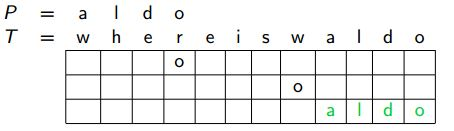
\includegraphics[scale=0.8]{bm1.jpg}
\end{center}
\end{figure}
\subsection{Good Suffix Examples}
\begin{figure}[ht]
\begin{center}
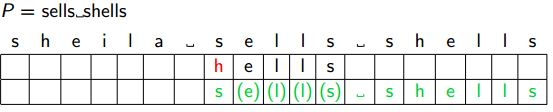
\includegraphics[scale=0.8]{BM2.jpg}
\end{center}
\end{figure}
\subsection{Last-Occurrence Function}
In order to utilize the previous two examples, we must \textit{preprocess} the pattern P and the alphabet $\Sigma$. We will build the \textit{last-occurrence function} L mapping $\Sigma$ to integers.\\
$L(c)$ is defined as:
\begin{itemize}
\item The largest index $i$ such that $P[i] = c$ or
\item $-1$ if no such index exists
\end{itemize}
\begin{ex}
Creating a Last-Occurrence function as shown in the course slides
\end{ex}
\begin{figure}[ht]
\begin{center}
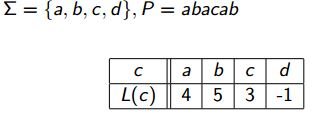
\includegraphics[scale=0.8]{lof.jpg}
\end{center}
\end{figure}
The runtime to build this function is $O(|\Sigma| + m)$ (we build an array of size $|\Sigma|$ and then we check every character in $P$ by doing $L[P[i]] = i$.
\subsection{Good Suffix Array}
Again, we \textit{preprocess} P to build a table. We create a \textbf{suffix skip array} S of size $m$: for $0 \leq i < m, S[i]$ is the largest index $j$ such that $P[i+1 ... m-1] = P[j+1 ... j + m - 1 - i]$ \textbf{and} $P[j] \neq P[i]$.
\begin{figure}[ht]
\begin{center}
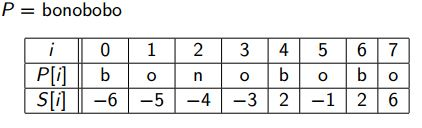
\includegraphics[scale=0.8]{suffix.jpg}
\end{center}
\end{figure}
This is computed in $\Theta(m)$ time.
%END%
\end{document}